\documentclass[a4paper,11pt,DIV=11,parskip=half]{scrartcl}

%%%%%%%%%%%%%%%%%%%%%%% Schrift und Sprache %%%%%%%%%%%%%%%%%%%%%%%%%%%%%%
\usepackage[ngerman]{babel}							% Sprachregeln für Deutsch
\usepackage[utf8]{inputenc}							% für Zeicheneingabe
\usepackage[T1]{fontenc}							% für Umlaute
\usepackage{lmodern}								% deutsche Trennungsregeln usw
%\usepackage{mathptmx}								% für Times New Roman
\usepackage{eurosym}								% für Euro Zeichen

%%%%%%%%%%%%%%%%%%%%%%% 	Seitenlayout	%%%%%%%%%%%%%%%%%%%%%%%%%%%%%%
%\usepackage[onehalfspacing]{setspace}				% 1,5 Zeilenabstand
\usepackage{setspace}								% für Zeilenabstand
\usepackage{scrlayer-scrpage}						% Für Kopf und Fußzeile
\pagestyle{headings}								% Seitenstil festlegen (z.B. Kopfzeile)
\clearpairofpagestyles								% Seitenstil löschen
\usepackage{float}									% um floats festen Platz zuweisen zu können (mit H)

%%%%%%%%%%%%%%%%%%%%%%% 	Tabellen		%%%%%%%%%%%%%%%%%%%%%%%%%%%%%%
\usepackage{multicol}								% Tabellenspalten verbinden
\usepackage{multirow}								% Tabellenzeilen verbinden
\usepackage{colortbl}								% Farben in Tabellen
\usepackage{tabularx}								% für Tabellenbreite
\usepackage{diagbox}								% für Schrägstriche in Tabellen

%%%%%%%%%%%%%%%%%%%%%%% 	Auflistung		%%%%%%%%%%%%%%%%%%%%%%%%%%%%%%
\usepackage{enumerate}								%
\usepackage{enumitem}								% für Listen
%\usepackage{outlines}								% Auflistung mit Stickpunkten (besser für Unterpunkte)

%%%%%%%%%%%%%%%%%%%%%%%		Mathematik		%%%%%%%%%%%%%%%%%%%%%%%%%%%%%%
\usepackage{siunitx}								% Si-Einheiten
\DeclareSIUnit{\belmilliwatt}{Bm}					% für Einheit dBm
\DeclareSIUnit{\dBm}{\deci\belmilliwatt}			% Einheit dBm
\sisetup{locale=DE}									% für Komma statt Punkt bei Zahlen
\usepackage{amsmath}								% Mathematik Umgebungen
\usepackage{amssymb}								% Mathematische Symbole und Zeichen
\usepackage{bm}										% Fette Schrift in Mathe Umgebung
\usepackage{amstext}								% Text in Matheumgebung
\usepackage{amsfonts}								% überflüssig, da in amssymb enthalten
\usepackage{empheq}									% Boxen z.B. mit align
\usepackage{mathtools}								% für senkrechtes "=" in newcommand
\usepackage{accents}								% für Akzente in Mathe "entspricht" in newcommand

%%%%%%%%%%%%%%%%%%%%%%%		Elektronik		%%%%%%%%%%%%%%%%%%%%%%%%%%%%%%
\usepackage{trfsigns}								% Transformationszeichen (z.B. Laplace-Zeit)

%%%%%%%%%%%%%%%%%%%%%%% 	Grafiken		%%%%%%%%%%%%%%%%%%%%%%%%%%%%%%
\usepackage{float}									% für Positionen von Bildern
\usepackage{wrapfig}								% Grafiken können neben Text stehen
\usepackage{color}									% Farben Paket für Zeichnungen
\usepackage{graphicx}								% Bilder können inkludiert werden
%\graphicspath{{E:/Studium/4_Semester}} 			% Pfad von dem Ordner von Bildern

%%%%%%%%%%%%%%%%%%%%%%% 	Zeichnungen		%%%%%%%%%%%%%%%%%%%%%%%%%%%%%%
\usepackage{pgfplots}          						% Diagramme erstellen
\pgfplotsset{compat=1.16}       					% Compatibilitätsmodus

\usepackage[siunitx,EFvoltages,european]{circuitikz}	% Schaltpläne

%%%%%%%%%%%%%%%%%%%%%%% 	Diagramme		%%%%%%%%%%%%%%%%%%%%%%%%%%%%%%
\usepackage{tikz,pgfplots}
\usetikzlibrary{math, calc, automata, positioning, arrows, intersections, shapes.geometric}

%\tikzset{
%	->, % makes the edges directed
	%		>=stealth’, % makes the arrow heads bold
	%	node distance=2.5cm, % specifies the minimum distance between two nodes. Change if necessary.
	%	every state/.style={thick, fill=gray!10}, % sets the properties for each ’state’ node
	%	initial text=$reset$, % sets the text that appears on the start arrow
%}

%%%%%%%%%%%%%%%%%%%%%%% 	KV-Diagramme	%%%%%%%%%%%%%%%%%%%%%%%%%%%%%%
%\usepackage{karnaugh}								% für KV-Diagramme
\usepackage{karnaugh-map}							% für KV-Diagramme
\usepackage{kvmap}									% für KV-Diagramme

%%%%%%%%%%%%%%%%%%%%%%% 	Codeeingabe		%%%%%%%%%%%%%%%%%%%%%%%%%%%%%%
\usepackage{minted}									% für Codehighlighting (z.B. VHDL)

%%%%%%%%%%%%%%%%%%%%%%% Quellenverzeichnis	%%%%%%%%%%%%%%%%%%%%%%%%%%%%%%
%\usepackage[style=science,backend=bibtex]{biblatex} % Für Quellenverzeichnis mit BibLatex
%\usepackage{filecontents}							% für festlegen von Quellen in der Tex Datei
%\addbibresource{NameDerDatei.bib}					% bindet die Quellen ein die vor documentclass 
% angelegt wurden

%%%%%%%%%%%%%%%%%%%%%%% 	für Befehle		%%%%%%%%%%%%%%%%%%%%%%%%%%%%%%
\usepackage{xparse}									% für \newcommand mit zwei optionalen Argumenten

%%%%%%%%%%%%%%%%%%%%%%% 	neue Pakete		%%%%%%%%%%%%%%%%%%%%%%%%%%%%%%


%%%%%%%%%%%%%%%%%%%%%%% 	eigene Befehle	%%%%%%%%%%%%%%%%%%%%%%%%%%%%%%%%%%%%%%%%%%%%%%%%%%%%%%%%%%%%%%%
%%%%%%%%%%%%%%%%%%%%%%% 	Laplace Symbol	%%%%%%%%%%%%%%%%%%%%%%%%%%%%%%
\newcommand{\vlaplace}{\mbox{\setlength{\unitlength}{0.1em}		% legt das Laplace Symbol vertikal als Bild
		\begin{picture}(20,10)									% an
			\put(1,-5){\circle*{4}}								% Laplace Seite unten
			\put(1,-3){\line(0,1){13}}
			\put(1,11){\circle{4}}
		\end{picture}							
	}
}
\newcommand{\vLaplace}{\mbox{\setlength{\unitlength}{0.1em}		% legt das Laplace Symbol vertikal als Bild
		\begin{picture}(20,10)									% an
			\put(1,-5){\circle{4}}								% Laplace Seite oben
			\put(1,-3){\line(0,1){13}}
			\put(1,11){\circle*{4}}
		\end{picture}							
	}
}
%%%%%%%%%%%%%%%%%%%%%%% 	Subsection		%%%%%%%%%%%%%%%%%%%%%%%%%%%%%%
\makeatletter													% um Probleme mit @ zu vermeiden (start)
\newcommand*{\addsubsec}{\secdef\@addsubsec\@saddsubsec}		% legt Makro addsubsec an
\newcommand*{\@addsubsec}{}										% schaut ob addsubsec noch nicht existiert
\def\@addsubsec[#1]#2{\subsection*{#2}\addcontentsline{toc}{subsection}{#1}		% definiert addsubsec
	%	\if@twoside\ifx\@mkboth\markboth\markright{#1}\fi\fi	% für wenn subsections im
	% Header stehen sollen
}
% \newcommand*{\@saddsubsec}[1]{\subsection*{#1}\@mkboth{}{}}	% für wenn subsections im
% Header stehen sollen
\makeatother													% um Probleme mit @ zu vermeiden (ende)

%%%%%%%%%%%%%%%%%%%%%%% 	Subsubsection	%%%%%%%%%%%%%%%%%%%%%%%%%%%%%%
\makeatletter													% um Probleme mit @ zu vermeiden (start)
\newcommand*{\addsubsubsec}{\secdef\@addsubsubsec\@saddsubsubsec}		% legt Makro addsubsubsec an
\newcommand*{\@addsubsubsec}{}									% schaut ob addsubsubsec noch nicht existiert
\def\@addsubsubsec[#1]#2{\subsubsection*{#2}\addcontentsline{toc}{subsubsection}{#1}		
	% definiert addsubsubsec
	%	\if@twoside\ifx\@mkboth\markboth\markright{#1}\fi\fi	% für wenn subsections im
	% Header stehen sollen
}
% \newcommand*{\@saddsubsec}[1]{\subsection*{#1}\@mkboth{}{}}	% für wenn subsections im
% Header stehen sollen
\makeatother													% um Probleme mit @ zu vermeiden (ende)

%%%%%%%%%%%%%%%%%%%%%%% Paragraph mit Linebreak	%%%%%%%%%%%%%%%%%%%%%%%%%%%%%%
%\makeatletter
%\renewcommand\paragraph{\@startsection{paragraph}{4}{\z@}%
%	{-2.5ex\@plus -1ex \@minus -.25ex}%
%	{1.25ex \@plus .25ex}%
%	{\normalfont\normalsize\bfseries}}
%\makeatother

\makeatletter													% um Probleme mit @ zu vermeiden (start)
\newcommand*{\addparagraphsec}{\secdef\@addparagraphsec\@saddparagraphsec}		% legt Makro addsubsubsec an
\newcommand*{\@addparagraphsec}{}								% schaut ob addsubsubsec noch nicht existiert
\def\@addparagraphsec[#1]#2{\paragraph*{#2}\addcontentsline{toc}{paragraph}{#1}%\mbox{}\\\\		
	% definiert addsubsubsec
	%	\if@twoside\ifx\@mkboth\markboth\markright{#1}\fi\fi	% für wenn subsections im
	% Header stehen sollen
}
% \newcommand*{\@saddsubsec}[1]{\subsection*{#1}\@mkboth{}{}}	% für wenn subsections im
% Header stehen sollen
\makeatother													% um Probleme mit @ zu vermeiden (ende)

\makeatletter
\newcommand*{\addparagraph}{\secdef\@addparagraph\@saddparagraph}
\newcommand*{\@addparagraph}{}
\def\@addparagraph[#1]#2{\addparagraphsec{#2}\mbox{}\\\\}
%\newcommand{\addparagraph}[1]{\addparagraphsec{#1}\mbox{}\\}
\makeatother

%%%%%%%%%%%%%%%%%%%%%%% 	Integral d		%%%%%%%%%%%%%%%%%%%%%%%%%%%%%%
\newcommand*\diff{\mathop{}\!\mathrm{d}}						% für das d beim Integral
\newcommand*\Diff[1]{\mathop{}\!\mathrm{d^#1}}					% für das d^(x) beim Integral

%%%%%%%%%%%%%%%%%%%%%%% senkrechtes Gleich	%%%%%%%%%%%%%%%%%%%%%%%%%%%%%%
\newcommand{\verteq}{\rotatebox{90}{$\,=$}}
\newcommand{\equalover}[2]{\overset{\scriptstyle\underset{\mkern4mu\verteq}{#2}}{#1}}

%%%%%%%%%%%%%%%%%%%%%%% "Entspricht"-Zeichen %%%%%%%%%%%%%%%%%%%%%%%%%%%%%
\newcommand{\eqvalent}[1]{\accentset{\wedge}{#1}}

%%%%%%%%%%%%%%%%%%%%%%% Tabular zweireihig  %%%%%%%%%%%%%%%%%%%%%%%%%%%%%%		
\NewDocumentCommand{\specialcell}{O{c} O{c} m m}{				% Zeilenumbruch in tabular-Umgebung
	\begin{tabular}[#1]{#2} {#3} \\ {#4}\end{tabular}}			% 1. [] t,c oder b 2. [] l,c oder r
%\newcommand{\specialcell}[4][c]{ 								% gleich wie oben, nur schlechter
	%	\begin{tabular}[#1]{@{}#2@{}}#3 \\ #4\end{tabular}}			% 

%%%%%%%%%%%%%%%%%%%%%%% 	neues Makro		%%%%%%%%%%%%%%%%%%%%%%%%%%%%%%

%%%%%%%%%%%%%%%%%%%%%%%%%%%%%%%%%%%%%%%%%%%%%%%%%%%%%%%%%%%%%%%%%%%%%%%%%%%%%%%%%%%%%%%%%%%%%%%%%%%%%%%%%%%
%%%%%%%%%%%%%%%%%%%%%%% 	Links			%%%%%%%%%%%%%%%%%%%%%%%%%%%%%%
\usepackage[hidelinks]{hyperref}					% Für Links auf Abschnitte usw ([] versteckt die Links)

%%%%%%%%%%%%%%%%%%%%%%%%%%%%%%%%%%%%%%%%%%%%%%%%%%%%%%%%%%%%%%%%%%%%%%%%%%%%%%%%%%%%%%%%%%%%%%%%%%%%%%%%%%%
%%%%%%%%%%%%%%%%%%%%%%% 	Quellen			%%%%%%%%%%%%%%%%%%%%%%%%%%%%%%
%\begin{filecontents}{NameDerDatei.bib}
%	@Book{NameDesFunktionsaufrufs,
	%		keywords = {},
	%		hyphenation = {},
	%		author = {},
	%		editor = {},
	%		translator = {},
	%		indextitle = {},
	%		title ={},
	%		shorttitle = {}}
%
%	@online{NameDesFunktionsaufrufs,
	%		label = {},
	%		title = {},
	%		year = {},
	%		url	= {},
	%		urldate = {}}
%\end{filecontents}
\setcounter{secnumdepth}{4}									% how many sectioning levels to assign numbers to
\setcounter{tocdepth}{4}									% how many sectioning levels to show in ToC

\begin{document}
	\pagenumbering{roman}
		\sffamily % Umschalten auf serifenlose Schrift für die Titelseite
	\parbox[t]{0.35\textwidth}
	{\vspace{0pt}\includegraphics[width=0.35\textwidth]{Bilder/HKA_Fakultät.jpg}}
	\hfill
	\parbox[t]{0.15\textwidth}
	{\vspace{0pt}
\includegraphics[width=0.15\textwidth]{Bilder/HKA_Logo.jpg}}
	\vfill
	\parbox{\textwidth}
	{\centering{
			{\Huge DDS}\\
			\rule{\textwidth}{1pt}\\[0.5ex]
			{\large Labor 4}}}
	\vfill
	\parbox{\textwidth}
	{\begin{flushright}{\large
			\begin{tabular}{rl}
				Studienfach:& EDS\\
				Dozent:& Prof. Dr.-Ing. Niclas Zeller\\
				Labor Durchführung:& Prof. Dr.-Ing. Niclas Zeller\\
				Bearbeiter:& Florian Ittensohn\\
				Matrikelnummer:& 66817\\
				E-Mail:& itfl1011@h-ka.de\\
				Studienvertiefung:& Informationstechnik\\
				Semester:& Sommersemester 2023\\
				&4. Semester \\
				Bearbeitet am:& 16.05.2023
			\end{tabular}}
	\end{flushright}}
	\rmfamily % Umschalten auf Serifenschrift
	\normalsize % Umschalten auf normale Größe
	\tableofcontents
	\newpage
	\ihead{\headmark}
	\automark{section}
	%	\ofoot{}
	%	\cfoot{}
	\ofoot{\pagemark}
	\pagenumbering{arabic}
%%%%%%%%%%%%%%%%%%%%%%%%%%%%%%%%%%%%%%%%%%% Vorbereitungsaufgaben %%%%%%%%%%%%%%%%%%%%%%%%%%%%%%%%%%%%%%%%%%%

%%%%%%%%%%%%%%%%%%%%%%%%%%%%%%%%%%%%%%%%%%%%    Laboraufgaben    %%%%%%%%%%%%%%%%%%%%%%%%%%%%%%%%%%%%%%%%%%%%
\section{Theoretische Vorbereitung}
Als Samplefrequenz soll $f_s$ = \SI{40}{kHz} und eine minimale Phasenschrittweite von \SI{1}{Hz}
angenommen werden.

\subsection{Funktionsweise einer DDS}
Bei einer DDS wird mit Hilfe eines Zählers, einer Look Up Table und anschließender Digital -> Analog Wandlung ein beliebiges Signal mit einem einzigen Oszillator realisiert. \\
Im Detail wird zunächst ein Zähler mit der maximal möglichen Auflösung und der minimalen Frequenz designed. Wenn dieser Modulozähler überläuft ist eine volle Periode des zu realisierenden Signals durchlaufen und der Zähler beginnt von vorne. \\
Zu jedem Schritt des Zählers gibt es eine korrespondierende Eintragung in der LUT mit dem zu dieser Phase gehörenden Signalwert. Dieser Signalwert ist der Ausgang unserer DDS.
\subsection{Nyquist-Shannon-Abtasttheorem}
Ein Signal mit der Frequenz $f_{signal}$ kann genau dann aus äquidistanten Abtastpunkten rekonstruiert werden, wenn die Abtastfrequenz $f_{abtast}$ folgende Bedingung erfüllt ist: 
\begin{equation}
	f_{abtast} >  2 \cdot  f_{signal}
\end{equation} 
\begin{figure}[H]
	\centering
	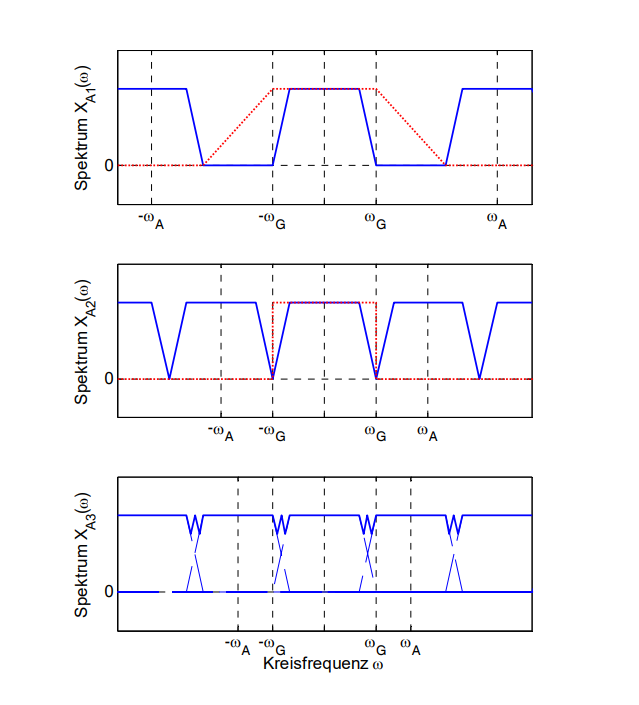
\includegraphics[width=0.6\textwidth]{Bilder/Nyquist_Shannon_Skizze.png}
	\caption{Skizze Nyquist Shannon Abtasttheorem}
	\label{fig:Nyquist_Shannon}
\end{figure}
\subsection{Bestimmen der Wortbreite des Phasenakkumulators}
Mit dem Phasenakkumulator soll bei einer minimalen Phasenschrittweite von \SI{1}{Hz} eine Spektrum zwischen \SI{1}{Hz} und \SI{10}{kHz} dargestellt werden. \\
Dazu müssen wir bei der höchsten Frequenz die Einhaltung des Nyquist-Shannon-Abtasttheorems beachten. Hier ergibt sich eine minimale Anzahl an Abtastpunkten zu:
\begin{equation}
	\begin{aligned}
	\SI{10}{kHz} \cdot 2 \text{ Punkte pro Periode } &\Rightarrow \text{ mind. } 20.000 \text{ Abtastpunkte bei \SI{1}{Hz}} \\
	\Rightarrow  ld(20.000) = 14.2877123795 &\Rightarrow \text{Wortbreite} = \SI{15}{bit}
	\end{aligned}
\end{equation}
\subsection{Phasenschritte}
\begin{table}[H]
	\centering
	\resizebox{0.4\textwidth}{!}{%
	\begin{tabular}{|l|l|}
	\hline
	Frequenz                          & Schrittweite  \\ \hline
	\SI{0}{Hz}                                & 0 oder 32.768 \\ \hline
	\SI{500}{Hz}   & 500           \\ \hline
	\SI{941}{Hz}   & 941           \\ \hline
	\SI{10000}{Hz} & 10000         \\ \hline
	\end{tabular}%
	}
	\end{table}

\subsection{Implementierung Phasenakkumulator}
\begin{figure}[H]
	\centering
	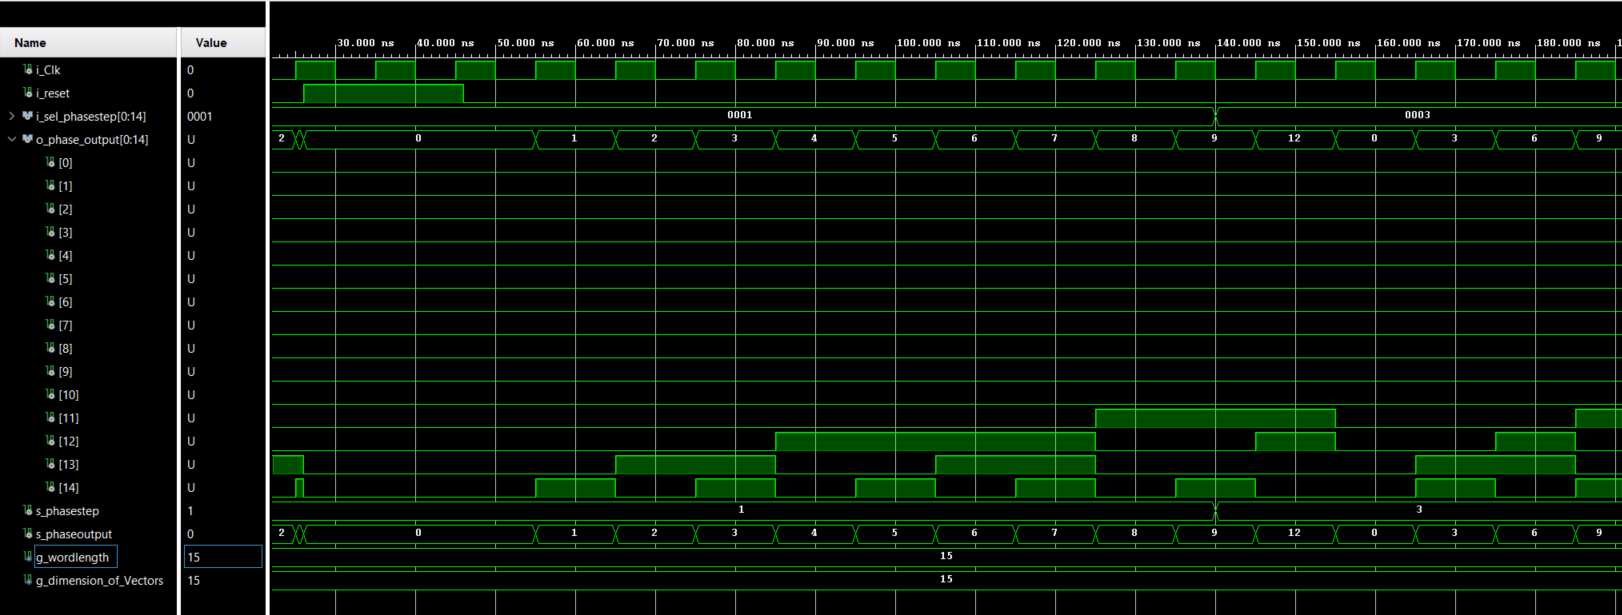
\includegraphics[width=\textwidth]{Bilder/Testbench_phaseincrement.png}
	\caption{Testbench für Phasenakkumulator}
	\label{fig:tb_Phaseaccu}
\end{figure}

\subsection{Welche Amplitudenauflösung ist sinnvoll?}
Da eine 15-Bit Auflösung in der Phase und damit auch der Zeit gewählt wurde ist es sinnvoll auch eine 15-Bit Auflösung in der Amplitude zu wählen. \\
Würde man beispielsweise eine deutlich kleinere Amplitudenauflösung als die Zeitauflösung wählen so wäre bei einer kontinuierlichen Funktion, wie sie hier beim Sinus vorliegt nur wenig zusätzliche Informatino verfügbar da das Signal sehr genau in der Zeit immer wieder dem gleichen ungenauen Amplitudenwert zugeordnet werden würde.
Einzig bei einer nicht kontinuierlichen Funktion wie z.B. einer Sägezahnspannung wäre es von Vorteil da man den Sprungpunkt besser eingrenzen könnte. 

\section{Implementierung und Analyse}
Hier das Pythonskript zum generieren der Werte.
\inputminted{python3}{../Labor4/Romgenerator_sine.py}
Für den Test wurde folgende Einstellung für den Phasesstep gesetzt: \\
\mint{VHDL}|v_phasesstep <= 0 after 5 ns, 500 after 1 ms, 941 after 10 ms, 10000 after 15 ms;|
\subsection{Verlauf \SI{0}{Hz}}
\begin{figure}[H]
	\centering
	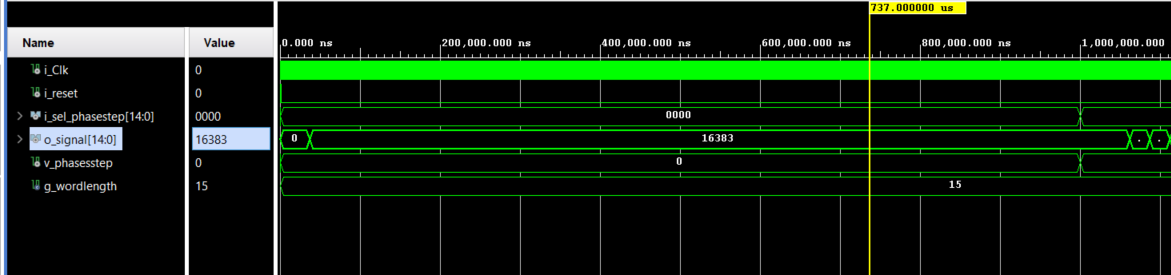
\includegraphics[width=\textwidth]{Bilder/DDS_0Hz.png}
	\caption{Verlauf \SI{0}{Hz}}
	\label{fig:tb_0Hz}
\end{figure}
\subsection{Verlauf \SI{500}{Hz}}
\begin{figure}[H]
	\centering
	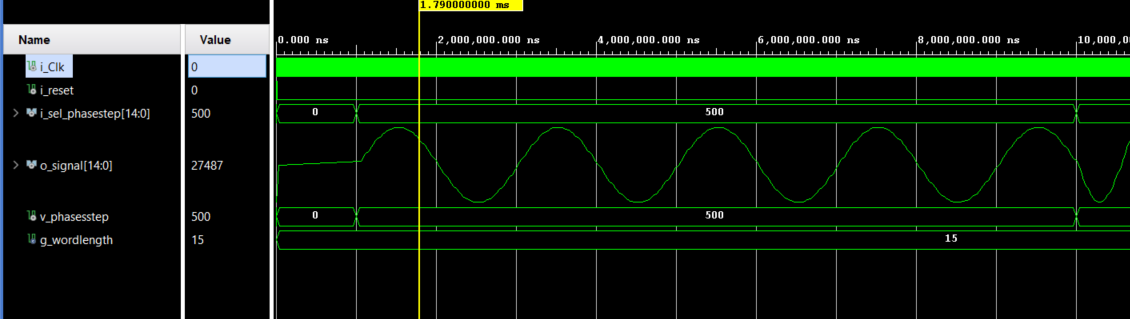
\includegraphics[width=\textwidth]{Bilder/DDS_500Hz.png}
	\caption{Verlauf \SI{500}{Hz}}
	\label{fig:tb_500Hz}
\end{figure}
\subsection{Verlauf \SI{941}{Hz}}
\begin{figure}[H]
	\centering
	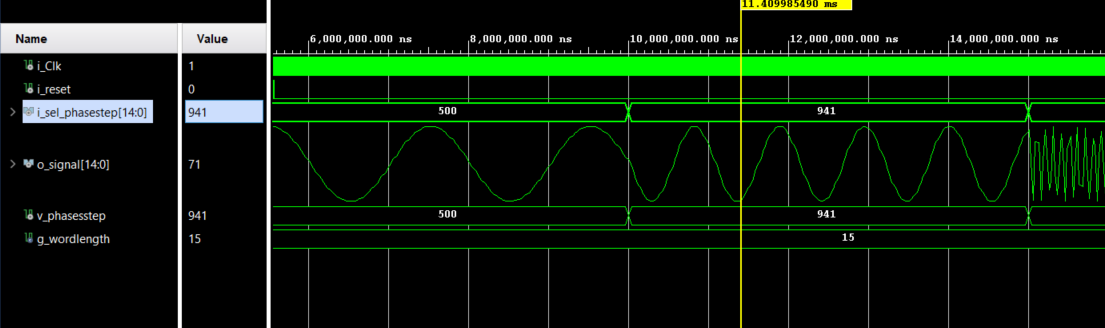
\includegraphics[width=\textwidth]{Bilder/DDS_941Hz.png}
	\caption{Verlauf \SI{941}{Hz}}
	\label{fig:tb_941Hz}
\end{figure}
\subsection{Verlauf \SI{10000}{Hz}}
\begin{figure}[H]
	\centering
	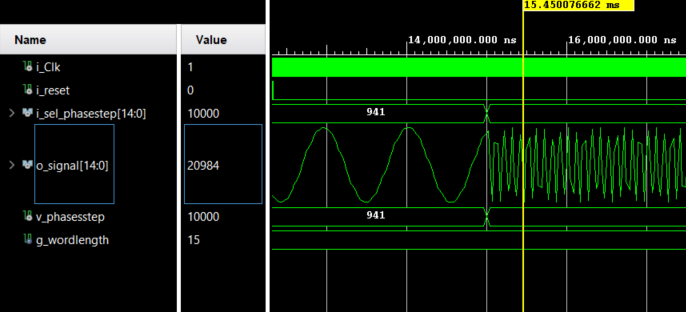
\includegraphics[width=\textwidth]{Bilder/DDS_10000Hz.png}
	\caption{Verlauf \SI{10000}{Hz}}
	\label{fig:tb_10000Hz}
\end{figure}
\subsection{Gesamtverlauf \SI{10000}{Hz}}
\begin{figure}[H]
	\centering
	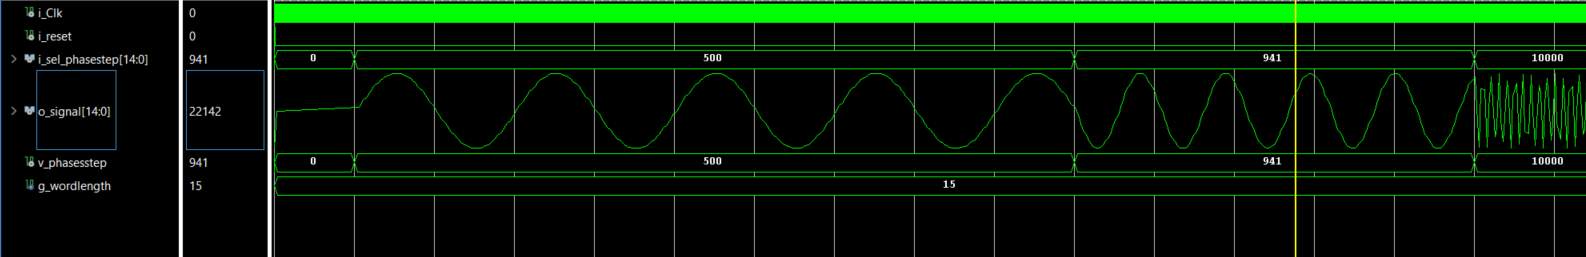
\includegraphics[width=\textwidth]{Bilder/DDS_gesamt.png}
	\caption{Gesamtverlauf}
	\label{fig:tb_DDS_alles}
\end{figure}
\paragraph*{Welche Besonderheiten treten bei \SI{0}{Hz} und \SI{941}{Hz} auf?}
Bei \SI{0}{Hz} wird konstant der selbe Wert gepusht. Bei \SI{941}{Hz} gibt es keine Besonderheit.
\section{PWM Vorbereitungsaufgaben}
\subsection{Funktionsweise PDM}
Eine PDM (Pulsdauermodulation) arbeitet mit einem festen Maximalwert für den Pegel des Signals und einer an die Periodendauer angepassten Ein- bzw. Auschaltzeit. Bei voller Aussteuerung wird über die ganze Periode das Ausgangssigal ausgegeben, dies entspricht einer Einstellung von 100 \%. 
Wenn ein geringer Signalwert ausgegeben werden soll ist die Einschaltzeit ensprechend ein gerignerer Teil der Periodendauer. \\
Im vorliegenden Fall wird die Dauer der Einschaltzeit mittels eines Vergleichs des auszugebenden Signals und einem Sägezahnsignal ermittelt. Wenn der Wert des Referenzsignals geringer als der Wert der Sägezahnspannung ist wird kein Ausgangssignal gegeben, wenn der Wert des Eingangssignals größer als der des Sägezahnsignals ist wird der Maximalwert ausgegeben. \\
Im Anschluss wird das Digitale Ausgangssignal mit einem Tiefpass "interpoliert".
\subsection{Analoge Realisierung einer PDM}
Ein Schmitt Trigger kann zur Realisierung einer PDM mit analogen Bauteilen gewählt werden.
\subsection{Frequenz für Phasenakkumulator}
Die minimale Frequenz des Phasenakkumulators für die Sägezahnspannung hängt von der gewählten Amplitudenauflösung und der maximalen Signalfrequenz ab. \\
Da eine symmetrische Amplitudenauflösung gewählt wurde muss im schnellsten Fall von \SI{10}{kHz} jeder Schritt der Amplitudenauflösung innerhalb einer Periode des Sägezahns durchlaufen werden.
Damit benötigen wir 32768 Schritte innerhalb einer Halteperiode des Eingangssignals der PWM. Die Dauer der Halteperiode ist abhängig von der Aktualisierungsfrequenz der Referenzsignals \SI{40}{kHz}. \\ Um die oben gewählte symmetrische Amplitudenauflösung zu bekommen würde eine Frequenz von $(2^{15})^2$ benötigt was größer als die Taktfrequenz des Boards ist. Deshalb wird die Taktfrequenz des Boards als Antriebsfrequenz des Phasenakkumulators der PWM gewählt, wodurch sich die Amplitudenauflösung vom optimalen Wert verschlechtert. 
Die neue Amplitudenauflösung beträgt: floor(32768/13) = 250 \\
Zudem berechnen wir die Schrittweite die einzustellen ist indem wir die Gesamtzahl der abzudeckenden Vergleichswerte durch das Verhältnisses der Periodendauer der Abtastfrequenz zur gewählten Clock des Boards.
\begin{align}
	\frac{2^{15}\cdot \SI{40}{kHz}}{\SI{100}{MhH}} = 13.107
\end{align}
\begin{figure}[H]
	\centering
	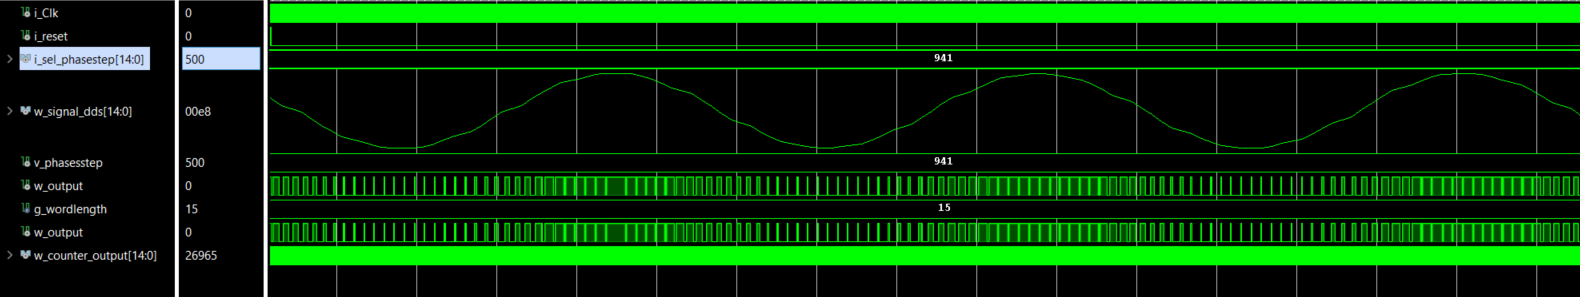
\includegraphics[width=\textwidth]{Bilder/DDS_FULL_PWM.png}
	\caption{Gesamtverlauf mit PWM}
	\label{fig:tb_DDS_PWM}
\end{figure}
\begin{figure}[H]
	\centering
	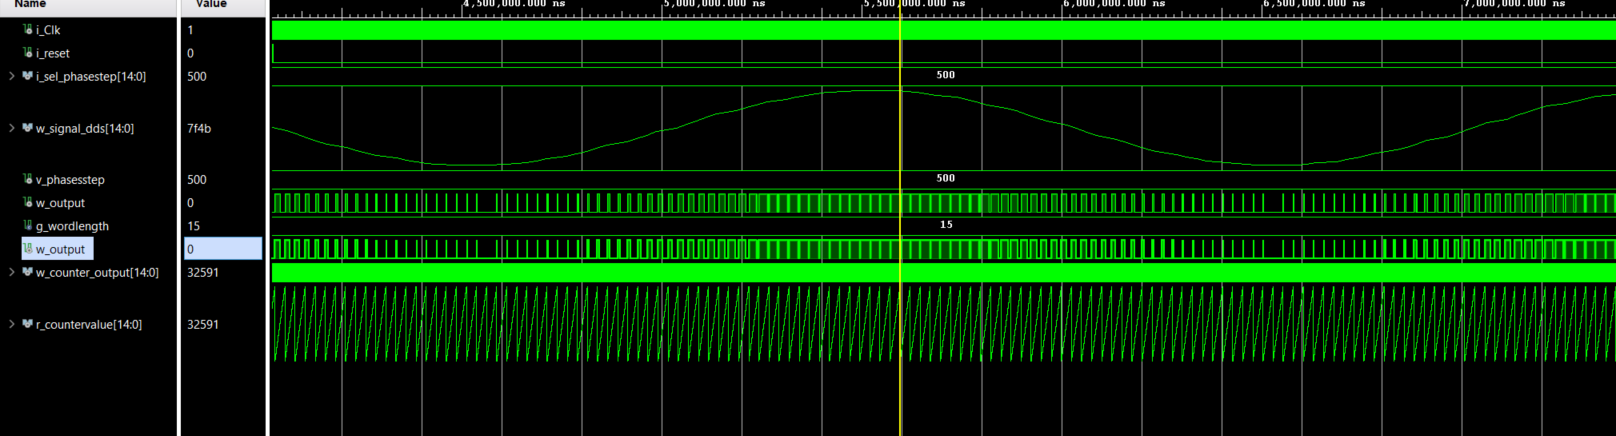
\includegraphics[width=\textwidth]{Bilder/DDS_FULL_PWM2.png}
	\caption{Gesamtverlauf mit PWM - Variante mit Sägezahnsignal}
	\label{fig:tb_DDS_PWM2}
\end{figure}
\begin{figure}[H]
	\centering
	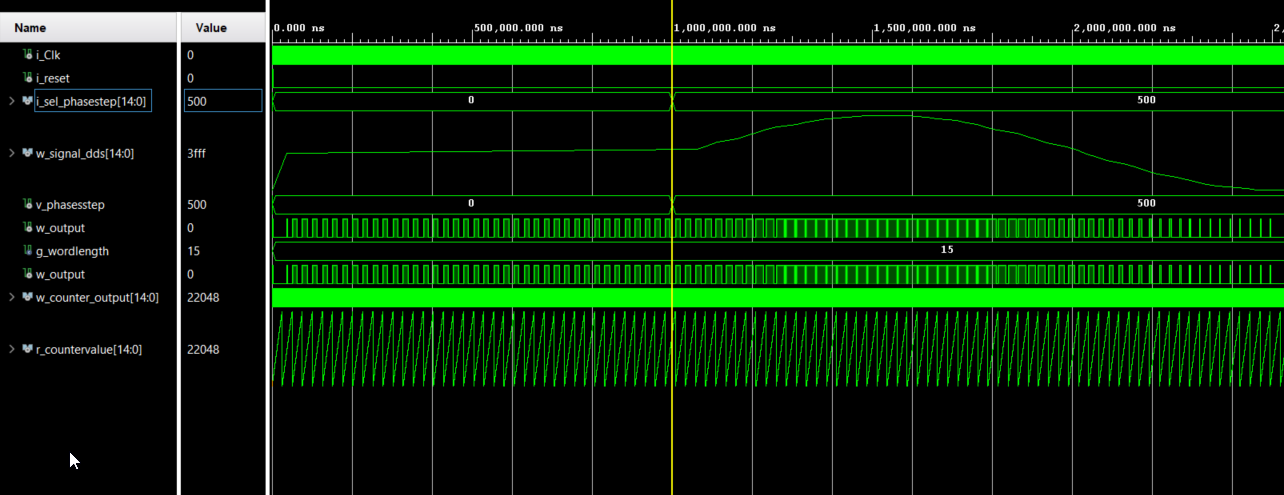
\includegraphics[width=\textwidth]{Bilder/Signalgenerator_0.png}
	\caption{Signalgenerator 0 Herz mit Übergang zu 500 Hz}
	\label{fig:tb_DDS_PWM3}
\end{figure}
\begin{figure}[H]
	\centering
	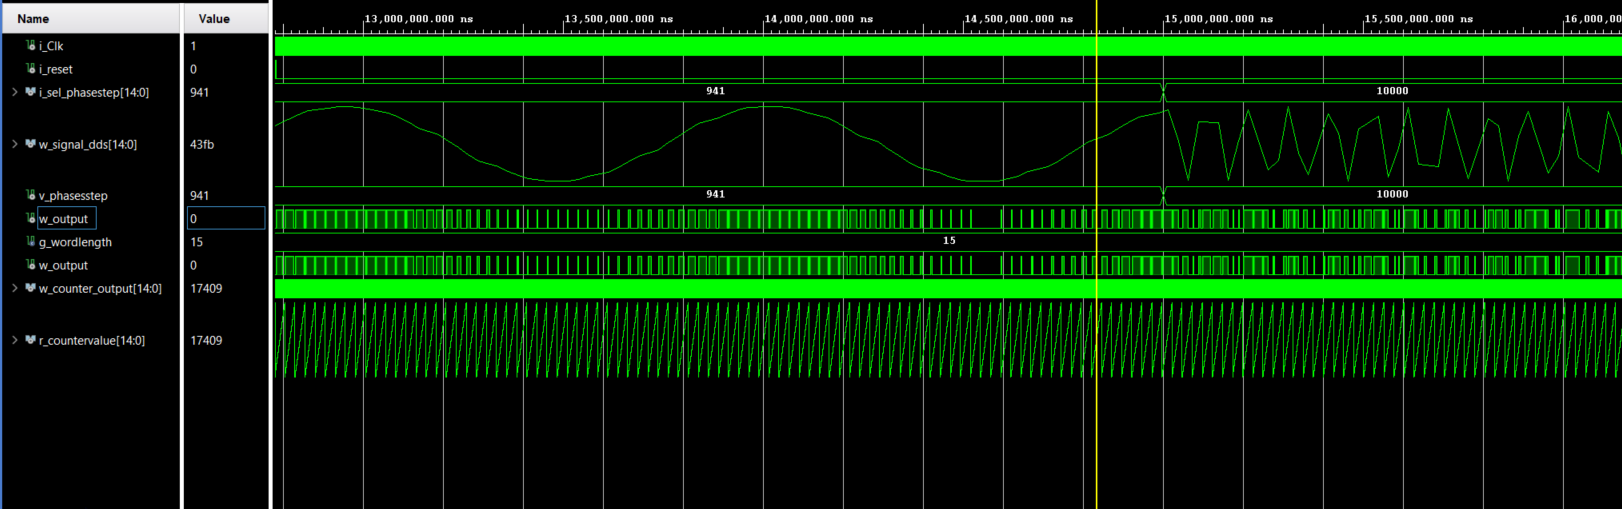
\includegraphics[width=\textwidth]{Bilder/Signalgenerator_941_10000.png}
	\caption{Signalgenerator \SI{941}{Hz} mit Übergang bis \SI{10}{kHz}}
	\label{fig:tb_DDS_PWM4}
\end{figure}


%%%%%%%%%%%%%%%%%%%%%%%%%%%%%%%%%%%%%%%%%%%%   Übersicht-Liste   %%%%%%%%%%%%%%%%%%%%%%%%%%%%%%%%%%%%%%%%%%%%
%%%%%%%%%%					Vorbereitungsaufgaben					%%%%%%%%%%


%%%%%%%%%%						Laboraufgaben						%%%%%%%%%%
% Aufgabe_3_1			ist erledigt
% Aufgabe_3_2			erledigt
% Aufgabe_3_3_1			erledigt
% Aufgabe_3_3_2			erledigt
% Aufgabe_3_3_3			erledigt
% Aufgabe_3_3_4			erledigt
% Aufgabe_3_3_5			erledigt
% Aufgabe_3_4_1			erledigt
% Aufgabe_3_4_2			erledigt
% Aufgabe_3_4_3			erledigt
% Aufgabe_3_5_1			erledigt
% Aufgabe_3_5_2			weiß ich nicht mehr
% Aufgabe_3_5_3_a		fertig
% Aufgabe_3_5_3_b		fertig
% Aufgabe_3_5_3_c		fertig
% Aufgabe_3_5_3_d		fertig
% Aufgabe_3_5_3_e		fertig

%%%%%%%%%%%%%%%%%%%%%%%%%%%%%%%%%%%%%%%%%%%%%%%%%%%%%%%%%%%%%%%%%%%%%%%%%%%%%%%%%%%%%%%%%%%%%%%%%%%%%%%%%%%%%
\end{document}